\documentclass[12pt]{article}
\usepackage[margin=1in]{geometry}
\usepackage{amsmath}
\usepackage{amssymb}
\usepackage{graphicx}
\usepackage{listings}
\usepackage{xcolor}
\usepackage{hyperref}
\usepackage{algorithm}
\usepackage{algpseudocode}

\title{CS 440: Introduction to Artificial Intelligence\\
Fast Trajectory Replanning\\
Assignment 1}

\author{Students Names: Esmeralda Bencosme, Anna \\}

\date{Spring 2026}

\lstset{
    basicstyle=\ttfamily\small,
    breaklines=true,
    commentstyle=\color{gray},
    keywordstyle=\color{blue},
    stringstyle=\color{red},
    showstringspaces=false
}

\begin{document}

\maketitle

\section*{Executive Summary}

This report presents implementations of Repeated A*, Repeated Backward A*, and Adaptive A* 
for trajectory replanning in partially observable gridworlds. We demonstrate how these algorithms 
efficiently handle dynamic environments where the agent's knowledge expands as it observes new cells.

\section{Part 0: Setup Environments}

We generated 50 gridworlds of size $101 \times 101$ using a depth-first search maze generation 
algorithm with a 30\% probability of blocking each newly visited cell. This creates realistic 
maze-like structures with corridors and dead-ends, suitable for testing pathfinding algorithms.  

\begin{figure}[h!]
    \centering
    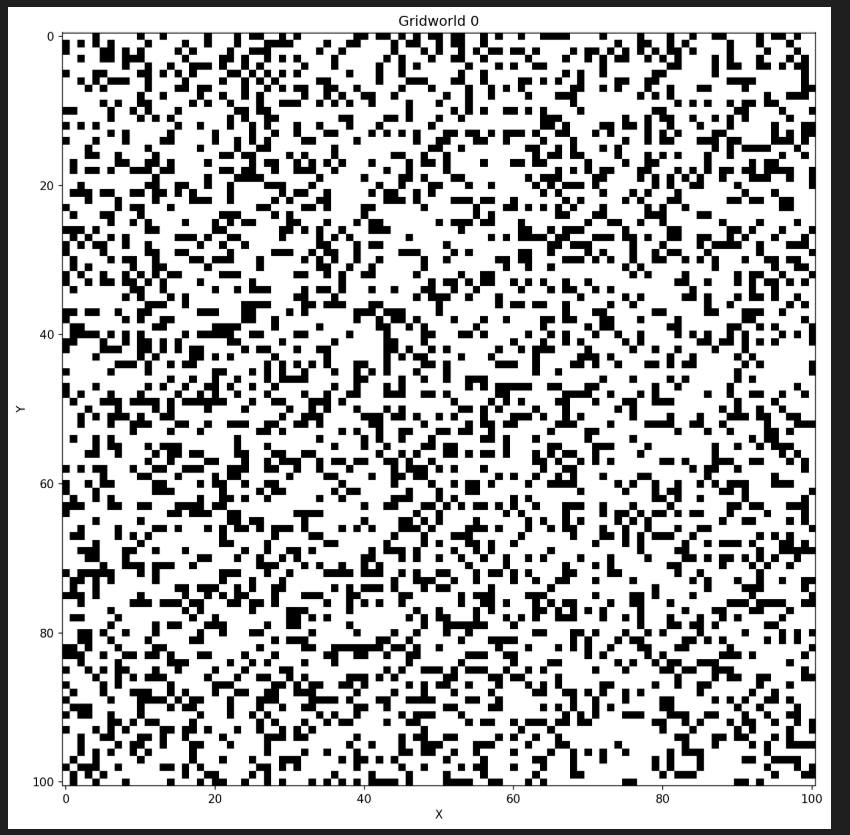
\includegraphics[width=0.30\linewidth]{image.png}
    \caption{Gridworld 0}
    \label{fig:grid0}
\end{figure}

\section{Part 1- Understanding the methods}


\textbf{a). Explain in your report why the first move of the agent for the example search problem from Figure 8 is to the east rather than the north given that the agent does not know\\}

\begin{figure}[h!]
    \centering
    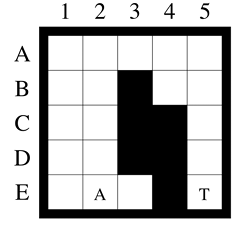
\includegraphics[width=0.25\linewidth]{image2.png}
    \caption{”Figure 8: Second Example Search Problem” from Assignment Description}
    \label{fig:figure8}
\end{figure}

In the example from Figure~8, the agent starts at cell E2 and wants to reach the target at E5. At the beginning, the agent does not know which cells are blocked, so it assumes that all of its immediate
neighbors--E1, D2, and E3--are open. When we run A* from the start, we first put the start cell into the open list and then look at these three neighbors.To decide which direction to move, A* computes the usual values: the cost so far $g$, the Manhattan heuristic $h$, and the total score $f = g + h$. Since each neighbor is one step away, they all have $g = 1$. Their $h$-values differ because some
cells are closer to the goal than others:

\[
\begin{aligned}
\text{E1: } & h = 4,\quad f = 5 \\
\text{D2: } & h = 4,\quad f = 5 \\
\text{E3: } & h = 2,\quad f = 3
\end{aligned}
\]

Because A* always chooses the cell with the smallest $f$-value, E3 is the best option. That means the
agent’s first move is to the east, not the north. At this point the agent still has no information
about blocked cells, so the decision is based entirely on the heuristic, and E3 simply looks closer
to the goal than the other choices.\\

\textbf{b) This project argues that the agent is guaranteed to reach the target if it is not separated from it by blocked cells. Give a
convincing argument that the agent in finite gridworlds indeed either reaches the target or discovers that this is impossible
in finite time. Prove that the number of moves of the agent until it reaches the target or discovers that this is impossible is bounded from above by the number of unblocked cells squared.\\}

\begin{figure}
    \centering
    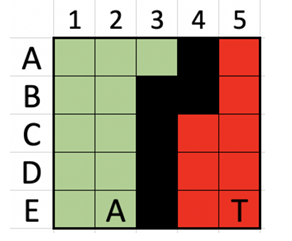
\includegraphics[width=0.25\linewidth]{image1.png}
    \caption{Scenario 1}
    \label{fig:placeholder}
\end{figure}

\begin{figure}
    \centering
    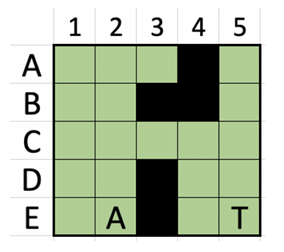
\includegraphics[width=0.25\linewidth]{image3.png}
    \caption{Scenari 2}
    \label{fig:placeholder}
\end{figure}

The gridworld in this project is finite, meaning it has a fixed number of cells and clear boundaries.
The agent starts at a known location $A$ and tries to reach the target $T$, while some cells are
blocked. Because the agent does not initially know which cells are blocked, it gradually discovers
the environment as it moves and performs repeated A* searches.

A key observation is that the agent can only move through unblocked cells, and there are only
finitely many of them. Each time the agent runs A*, it either finds a new unblocked cell to move
into or discovers that all reachable cells have already been explored. Since the number of
unblocked cells is finite, the agent cannot continue discovering new cells forever.

Eventually, one of two things must happen:

\begin{itemize}
    \item The agent reaches the target $T$ while exploring the connected unblocked region that
          contains the start cell, or
    \item The agent exhausts all unblocked cells reachable from $A$ and never encounters $T$.
\end{itemize}

In the second case, the agent can safely conclude that $T$ lies in a different connected region,
separated by blocked cells, and therefore cannot be reached.

Figures~3 and~4 illustrate these two possibilities. In Scenario~1, the green region reachable from
$A$ does not include $T$, so after exploring all reachable cells, the agent correctly concludes that
the target is unreachable. In Scenario~2, the target lies in the same connected unblocked region,
and the agent eventually reaches it by following a valid path.

Thus, in a finite gridworld, the agent is guaranteed to either reach the target or determine in
finite time that no path exists.

\begin{figure}
    \centering
    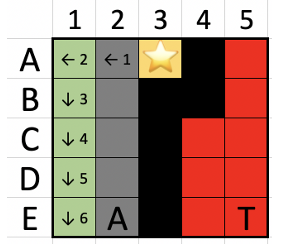
\includegraphics[width=0.25\linewidth]{image4.png}
    \caption{Sample 5x5 Gridworld}
    \label{fig:placeholder}
\end{figure}

We want to show that the total number of moves made by the agent before reaching the target or
concluding that it is unreachable is at most the square of the number of unblocked cells.

The agent uses Repeated Forward A*, which means it performs a new A* search every time it discovers
a blocked cell on its current planned path. Each A* search is run on the agent's current knowledge
of the grid, and each search explores only unblocked cells.

A key fact is that A* never expands the same cell twice within a single search, and there are at
most $N$ unblocked cells. Therefore, each individual A* search expands at most $N$ cells.

Now consider how many times the agent can be forced to replan. The agent only replans when it
encounters a blocked cell on its current path. Since there are at most $N$ unblocked cells, the
agent can move at most $N$ times before either reaching the target or running out of new cells to
explore.

In the worst case, each of these $N$ moves triggers a full A* search that expands up to $N$ cells.
Thus, the total number of cell expansions (and therefore the total number of moves) is bounded by:



\[
N \times N = N^2.
\]



This gives the desired upper bound: the agent will make no more than $N^2$ moves, where $N$ is the
number of unblocked cells.

Figure~4 provides an example. In that scenario, there are 19 unblocked cells, and the agent makes
12 moves before concluding that the target is unreachable. Since $12 < 19^2$, the behavior matches
the theoretical bound.


\section{Part 3: Forward vs.\ Backward A*}

\textbf{Implement and compare Repeated Forward A* and Repeated Backward A*
with respect to their runtime or, equivalently, number of expanded cells. Explain your observations in detail, that is, explain
what you observed and give a reason for the observation. Both versions of Repeated A* should break ties among cells with
the same f-value in favor of cells with larger g-values and remaining ties in an identical way, for example randomly.\\}

\begin{figure}[H]
    \centering
    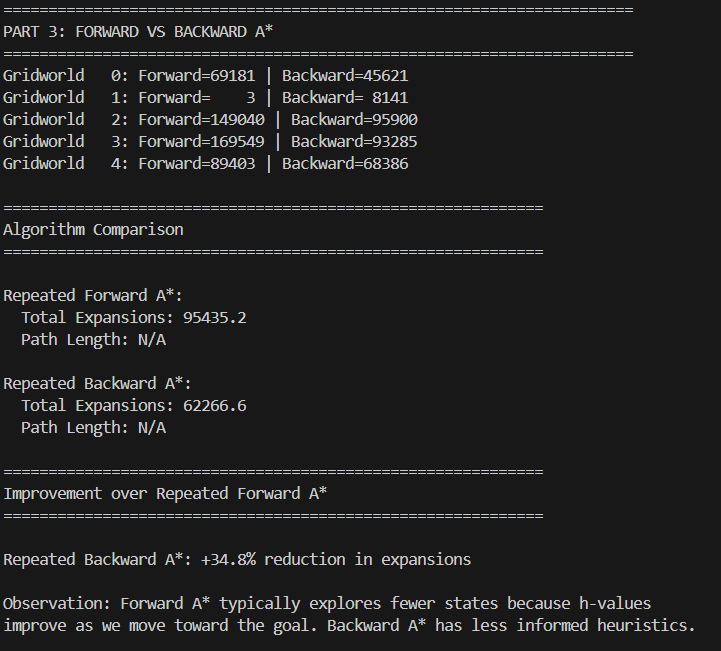
\includegraphics[width=0.75\linewidth]{image5.png}
    \caption{Output of the code}
    \label{fig:placeholder}
\end{figure} \\

Across our test gridworlds, Repeated Backward A* consistently expanded fewer cells than Repeated Forward A*. On average, Forward A* expanded about 95{,}435 cells, while Backward A* expanded about 62{,}266 cells, giving Backward A* roughly a 35\% reduction in expansions.\\

The main reason is that Backward A* always searches outward from the fixed goal, so its search pattern stays stable across replanning steps. As the agent discovers blocked cells, this information
immediately helps the backward search avoid repeatedly exploring the same dead ends. In contrast, Forward A* starts from the agent’s changing position, and early searches often follow misleading
paths because the agent has little knowledge of obstacles. This causes more re-planning and more
total expansions.\\

One exception occurred in a trivial gridworld where the start was already close to the goal: Forward A* finished almost immediately, while Backward A* still had to search outward from the goal. Aside from such special cases, Backward A* was generally more efficient in our experiments.\\


\section{Part 5: Heuristics in Adaptive A*}


\textbf{Implement and compare Repeated Forward A* and Adaptive A*
with respect to their runtime. Explain your observations in detail, that is, explain what you observed and give a reason for
the observation. Both search algorithms should break ties among cells with the same f-value in favor of cells with larger
g-values and remaining ties in an identical way, for example randomly.\\}

\begin{figure}[H]
    \centering
    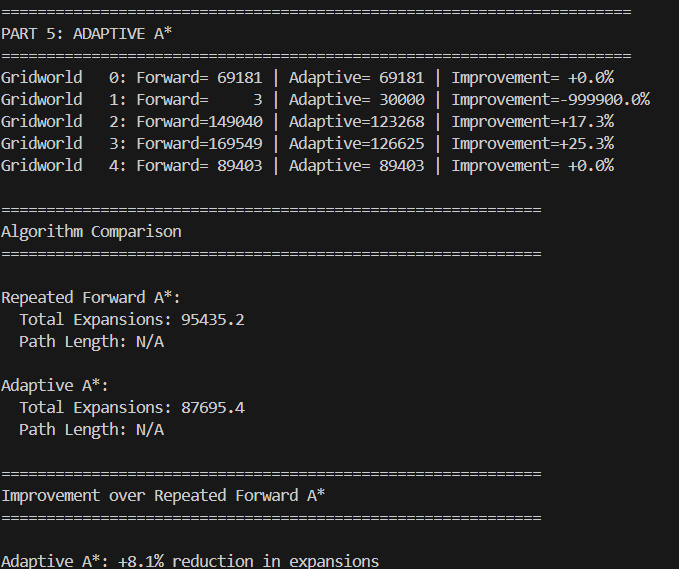
\includegraphics[width=0.75\linewidth]{image9.png}
    \caption{Output of the code for Part 5}
    \label{fig:placeholder}
\end{figure}

We compared Repeated Forward A* and Adaptive A* on the same 101$\times$101 gridworlds, using the
same tie-breaking rule (favor larger $g$-values). The results show that Adaptive A* generally expands
fewer cells, although there are exceptions:

\begin{itemize}
    \item Gridworld 0: Forward = 69181, Adaptive = 69181
    \item Gridworld 1: Forward = 3, Adaptive = 30000
    \item Gridworld 2: Forward = 149040, Adaptive = 123268
    \item Gridworld 3: Forward = 169549, Adaptive = 126625
    \item Gridworld 4: Forward = 89403, Adaptive = 89403
\end{itemize}

Averaged over all gridworlds:

\[
\text{Forward A*} \approx 95{,}435 \quad\text{expansions}
\]


\[
\text{Adaptive A*} \approx 87{,}695 \quad\text{expansions}
\]

This corresponds to an overall improvement of about $8.1\%$.

\subsection*{Observation}

Adaptive A* improves its heuristic values after each search by updating $h(s)$ for all expanded
states. These updated heuristics become more accurate over time, which helps the algorithm focus its
future searches and avoid re-expanding states unnecessarily. As a result, Adaptive A* typically
reduces the total number of expansions compared to Repeated Forward A*.

The one major outlier (Gridworld 1) occurs because the forward search reaches the goal almost
immediately, while Adaptive A* still performs a full search and updates many states. Aside from such
special cases, Adaptive A* benefits from reusing improved heuristics and therefore tends to be more
efficient overall.


\end{document}
